\chapter{Implementation}

\section{Storage}
Storage is the function of a backup system and we wanted to ensure that the storage mechanism we used would be reliable, secure, and maintainable. MySQL was a clear choice. It is well tested, contains an excellent permissions system, and is commercially supported. 
\subsection{Storage Layout}
Internally the database uses five different tables to store all data: clients, jobs, files, blocks, and logs. The "clients" table relates the IP address of the client to a client ID. The "jobs" table relates a job ID  with a time and a client. The file table relates file permissions and dates to a file ID. The blocks table stores all the file data in a series of blocks which are indexed by their SHA1 hash.

In order for the structure of the file system to be properly represented, we needed a way to relate files to each other to form a directed tree. This is provided by a file table that relates one file ID to another. While this table is sufficient to represent a graph of files, the file systems we back up are proper trees. Using this system has an added benefit: Files and directories can be represented using the same schema. Since both have identical collection of attributes, we use this system without any loss of information.

Jobs need to be related to a series of files to be backed up on the client machine. To do this, a table relating file IDs to job IDs is provided. As many file IDs as desired can be related to a given job ID.

The actual data contained in the files are stored in a table of blocks. Each block is of a fixed size and is indexed by its hash. The file metadata is related to a set of blocks through an intermediate table that relates file IDs to the hashes of the blocks that make up the file. The entries are inserted in the order that the blocks appear in the file.

\subsection{Storage Optimization}
Separating files into blocks allowed us to optimise the storage used. Many files share common parts, and duplicate blocks are simply not inserted into the system. In our tests, we got up to 30% compression on par with the GZIP compression algorithm.
\subsection{Insertion}
Once a client has been inserted, a job has been created, and the job has been related to the directories the user wants to back up, the inserter uses the SFTP protocol to connect to the client system at the IP stored in the clients table. It logs into the system using a predefined password. It then recursively compares the record for each directory, updating file entries that already exist and inserting file records that do not exist. No file record is ever deleted.

\section{Distribution Algorithm}

In order to distribute the backup data across our network, our system uses a
peer-to-peer networking algorithm based on Content Addressable Networks. \cite{scalable}
The algorithm is centered around the concept of a hash table that is shared by all the backup
servers in the network. The hash table is modeled as a square, and the backed up files are then
points that are hashed into this square. Each backup server in the network owns a rectangular portion
of this square, and is responsible for storing all the files whose points map into this rectangle.
This concept is shown in Figure \ref{fig:dht_1}. In this figure, in order to retrieve file 8 from the server,
it has to be retrieved from backup server 2.

\begin{figure}[hb]
\centering
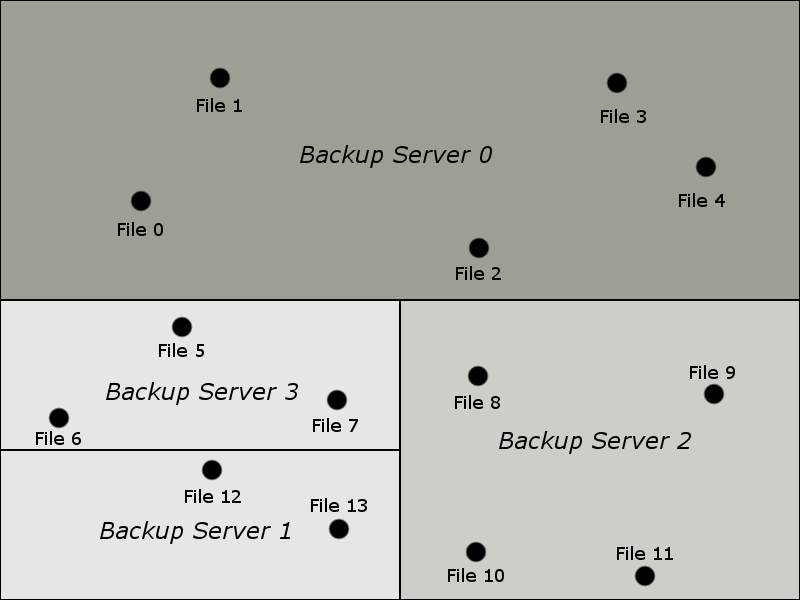
\includegraphics[scale=0.5]{images/dht_basic.png}
\caption{Distributed Hash Table}
\label{fig:dht_1}
\end{figure}

This algorithm has to take into account the fact that the network is chaotic and unstable.
Any backup server within the network can disappear from the network at any time and without warning.
Any backup server can also rejoin the network at any time. This is accounted for by the algorithm by
the way the network is structured. Each backup server in the network only communicates directly with
other servers that own a portion of the hash table adjacent to its own portion, called its neighbors.
For example, in Figure \ref{fig:dht_2}, backup server 2's neighbors are servers 4, 9, 3, and 8.

\begin{figure}[hb]
\centering
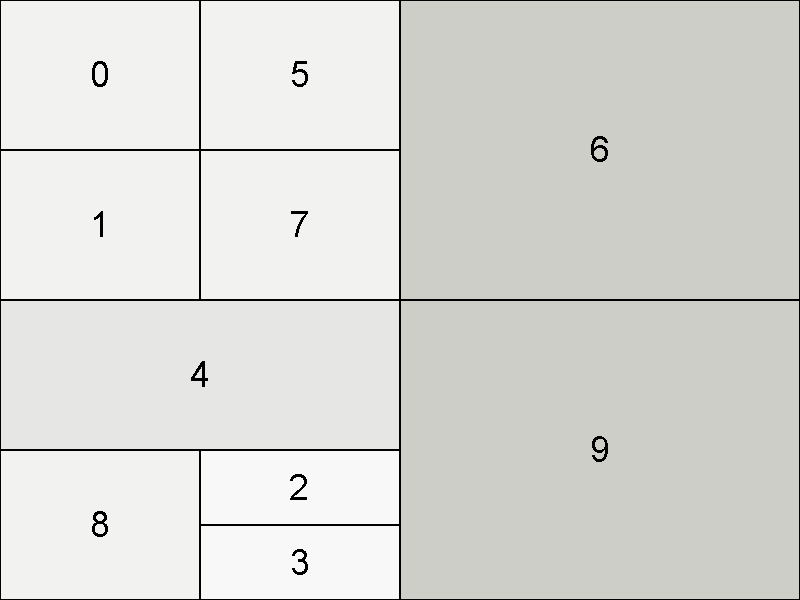
\includegraphics[scale=0.5]{images/dht_10_nodes.png}
\caption{Distributed Hash Table with 10 nodes}
\label{fig:dht_2}
\end{figure}

Then in order to deal with the fact that a backup server could disappear from the network at any time,
the neighbors of a backup server that goes down are responsible for taking over the space it occupied
in the hash table. Each backup server maintains consistent communication with its neighbors. If a server
is no longer responding to its neighbors, then those neighbors will negotiate to see who takes ownership
of the space the unresponsive server occupied in the hash table. In this way, each backup server is responsible
for maintaining the stability of the network near it in the hash table.
 


\section{Client-Server Discovery Procedure}
\begin{figure}
\centering
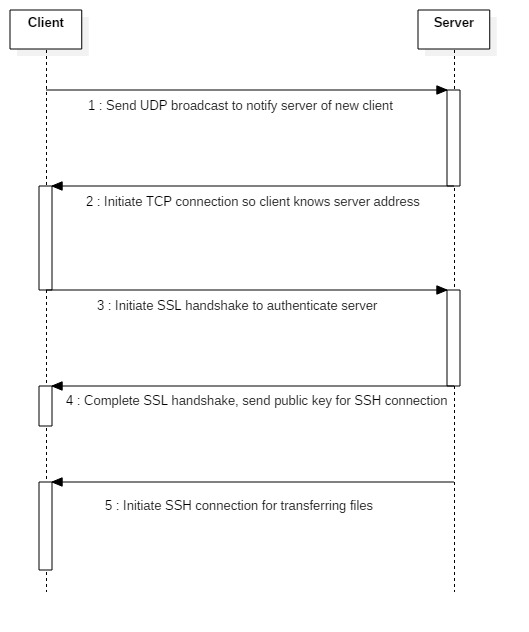
\includegraphics[scale=0.5]{images/SequenceDiagram1.jpg}
\caption{Client-Server Discovery Procedure}
\label{fig:connect}
\end{figure}

Once the user has already set up the server on their own LAN, they are ready to connect their own client machines to the system.  The user installs certain basic client software on their machine which, upon activation, sends out a UDP broadcast onto the network to notify the server of a new client.  Once the server receives the broadcast, it then initiates a TCP connection so that the client knows the proper server address to connect to.  The client then initiates an SSL handshake using the wolfSSL library, in order to verify that the server is a valid party and not just a listener on the network who wishes to intercept data.  This is made possible by each server possessing it's own unique private key, set at manufacture time, and signed by our central certifiate authority  The client program includes a public key that can verify that the server is who it says it is.  Once the ssl handshake is completed, the server sends a public key to the client which the client can use to recognize a legetimate openSSH connection.  In addition, at this point the client is given a private key used by the server to identify its unique user account for accessing files.  Now that both the client and the server possess valid credentials and information on each other, the server may then initiate ssh connections for transferring files.

\section{Web Configuration Interface}

Our Web Configuration Interface was a simple webpage, and so used the typical technologies of HTML, Javascript, and PHP.  IgniteUI was used to construct the interface.  PHP extensions were used to call various applications on the server in response to user inputs.